%%%%%%%%%%%%%%%%%%%%%%%%%%%%%%%%%%%%%%%%%%%%%%%%%%%%%%%%%%%%%%%%%%%%%%%%
\clearpage
\section{Functions for analysing azimuthal averaged data}


%%%%%%%%%%%%%%%%%%%%%%%%%%%%%%%%%%%%%%%%%%%%%%%%%%%%%%%%%%%%%%%%%%%%%%%%%

%\clearpage
\subsection{$\sin^2$-$\sin^4$ azimuthal analysis} ~\\
This plugin can be used to describe azimuthal averaged data in case of e.g.\ magnetic scattering \cite{Wiedenmann2011}, where depending on the incident and scattered polarization and the dipole-dipole nature of the interaction of the neutron with a magnetic moment of an atom an angle dependent cross-section is observed even though the scattering objects are spherical. The spherical symmetry is broken by orienting the magnetic towards a applied magnetic field. Some detailed form factor for magnetic objects can be found in chapter \ref{sec:magneticstructures}. The scattering can be often decomposed in an isotropic term independent of the angle between the scattering vector and the applied field and anisotropic terms which anisotropy term is described by a $\sin^2(\psi)$ and $\sin^4(\psi)$ term.
\begin{align}
I_\mathrm{rad}(\psi) &= A + B\sin^2(\psi-\delta) + C \sin^4(\psi-\delta) \\
I_\mathrm{deg}(\psi) &= A + B\sin^2\left((\psi-\delta)\frac{\pi}{180}\right) + C \sin^4\left((\psi-\delta)\frac{\pi}{180}\right)
\end{align}

\hspace{1pt}\\
\underline{Input Parameters for models \texttt{A+Bsin2+Csin4 (deg)} and \texttt{A+Bsin2+Csin4 (rad)}:}\\
\begin{description}
\item[\texttt{A}] isotropic scattering intensity $A$
\item[\texttt{B}] anisotropic $\sin^2$-dependent scattering intensity $B$
\item[\texttt{C}] anisotropic $\sin^4$-dependent scattering intensity $C$
\item[\texttt{delta}] direction of the polarisation $\delta$ in degree or radian
\end{description}

\underline{Note:}
None.


\begin{figure}[htb]
\begin{center}
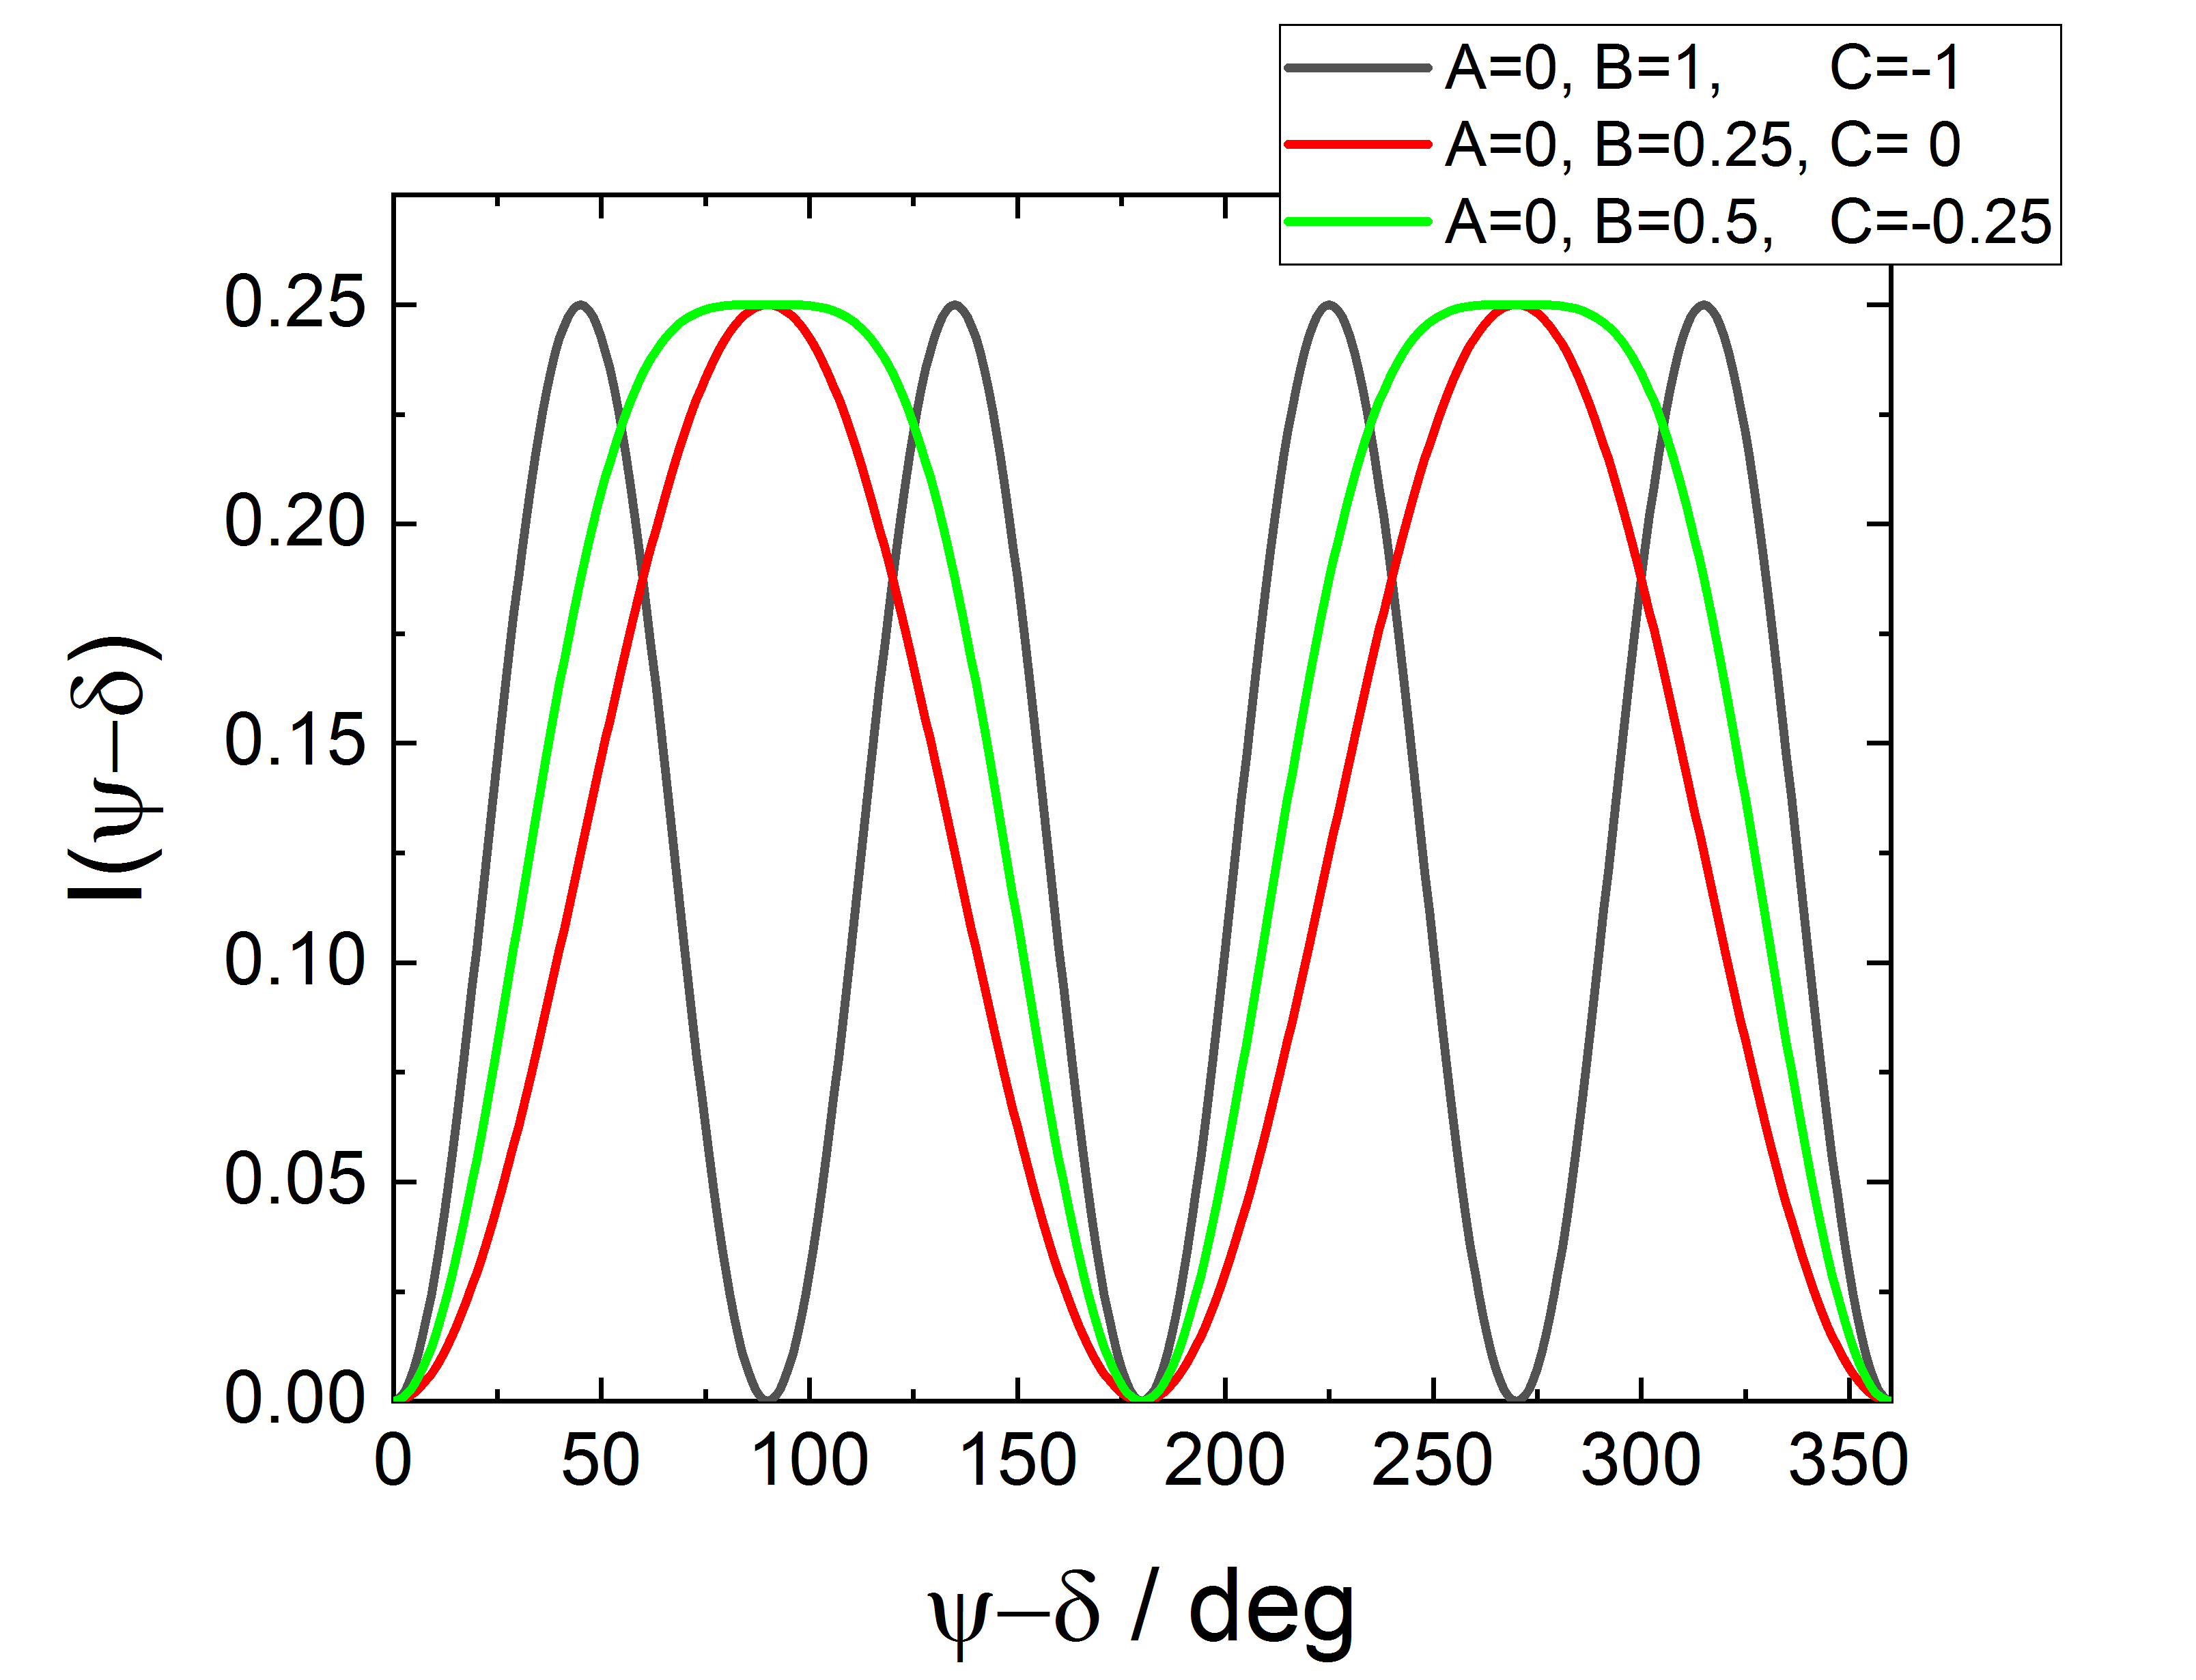
\includegraphics[width=0.7\textwidth]{../images/form_factor/azimuthal/sin2sin4.png}
\end{center}
\caption{Azimuthal intensity distribution typical in the field of magnetic scattering}
\label{fig:IQsin2sin4}
\end{figure}

\subsection{Maier-Saupe azimuthal analysis} ~\\
In the Picken model \cite{Picken1990,Fan1994,Makarova2013} the azimuthal intensity reads as
\begin{align}
  \mathcal{I}_\mathrm{P}(\chi) &= \exp\left(\kappa\cos^2\chi\right)\\
\chi &= \psi-\delta
\end{align}
The final model function is than normalized on the average intensity so that the azimuthal intensity distribution is given by
\begin{align}
  I_\mathrm{P}(\chi) &= I_0 + A \frac{\pi}{2}\frac{\mathcal{I}_\mathrm{P}(\chi)}{\int_0^{\pi/2}\mathcal{I}_\mathrm{P}(\chi)\mathrm{d}\chi}
\end{align}

\hspace{1pt}\\
\underline{Input Parameters for models \texttt{MaierSaupe (deg)} and \texttt{MaierSaupe (rad)}:}\\
\begin{description}
\item[\texttt{I0}] flat background $I_0$
\item[\texttt{A}] Amplitude $A$ of the angle dependent intensity
\item[\texttt{kappa}] parameter for strength of orientation $\kappa$
\item[\texttt{delta}] direction of the polarisation $\delta$ in degree or radian
\end{description}

\underline{Note:}
For $\kappa=0$ the azimuthal intensity is flat, for $\kappa>0$ the highest intensity is in the direction $\psi-\delta=0$ and for $\kappa<0$ in the direction $\psi-\delta=\pi/2$

\begin{figure}[htb]
\begin{center}
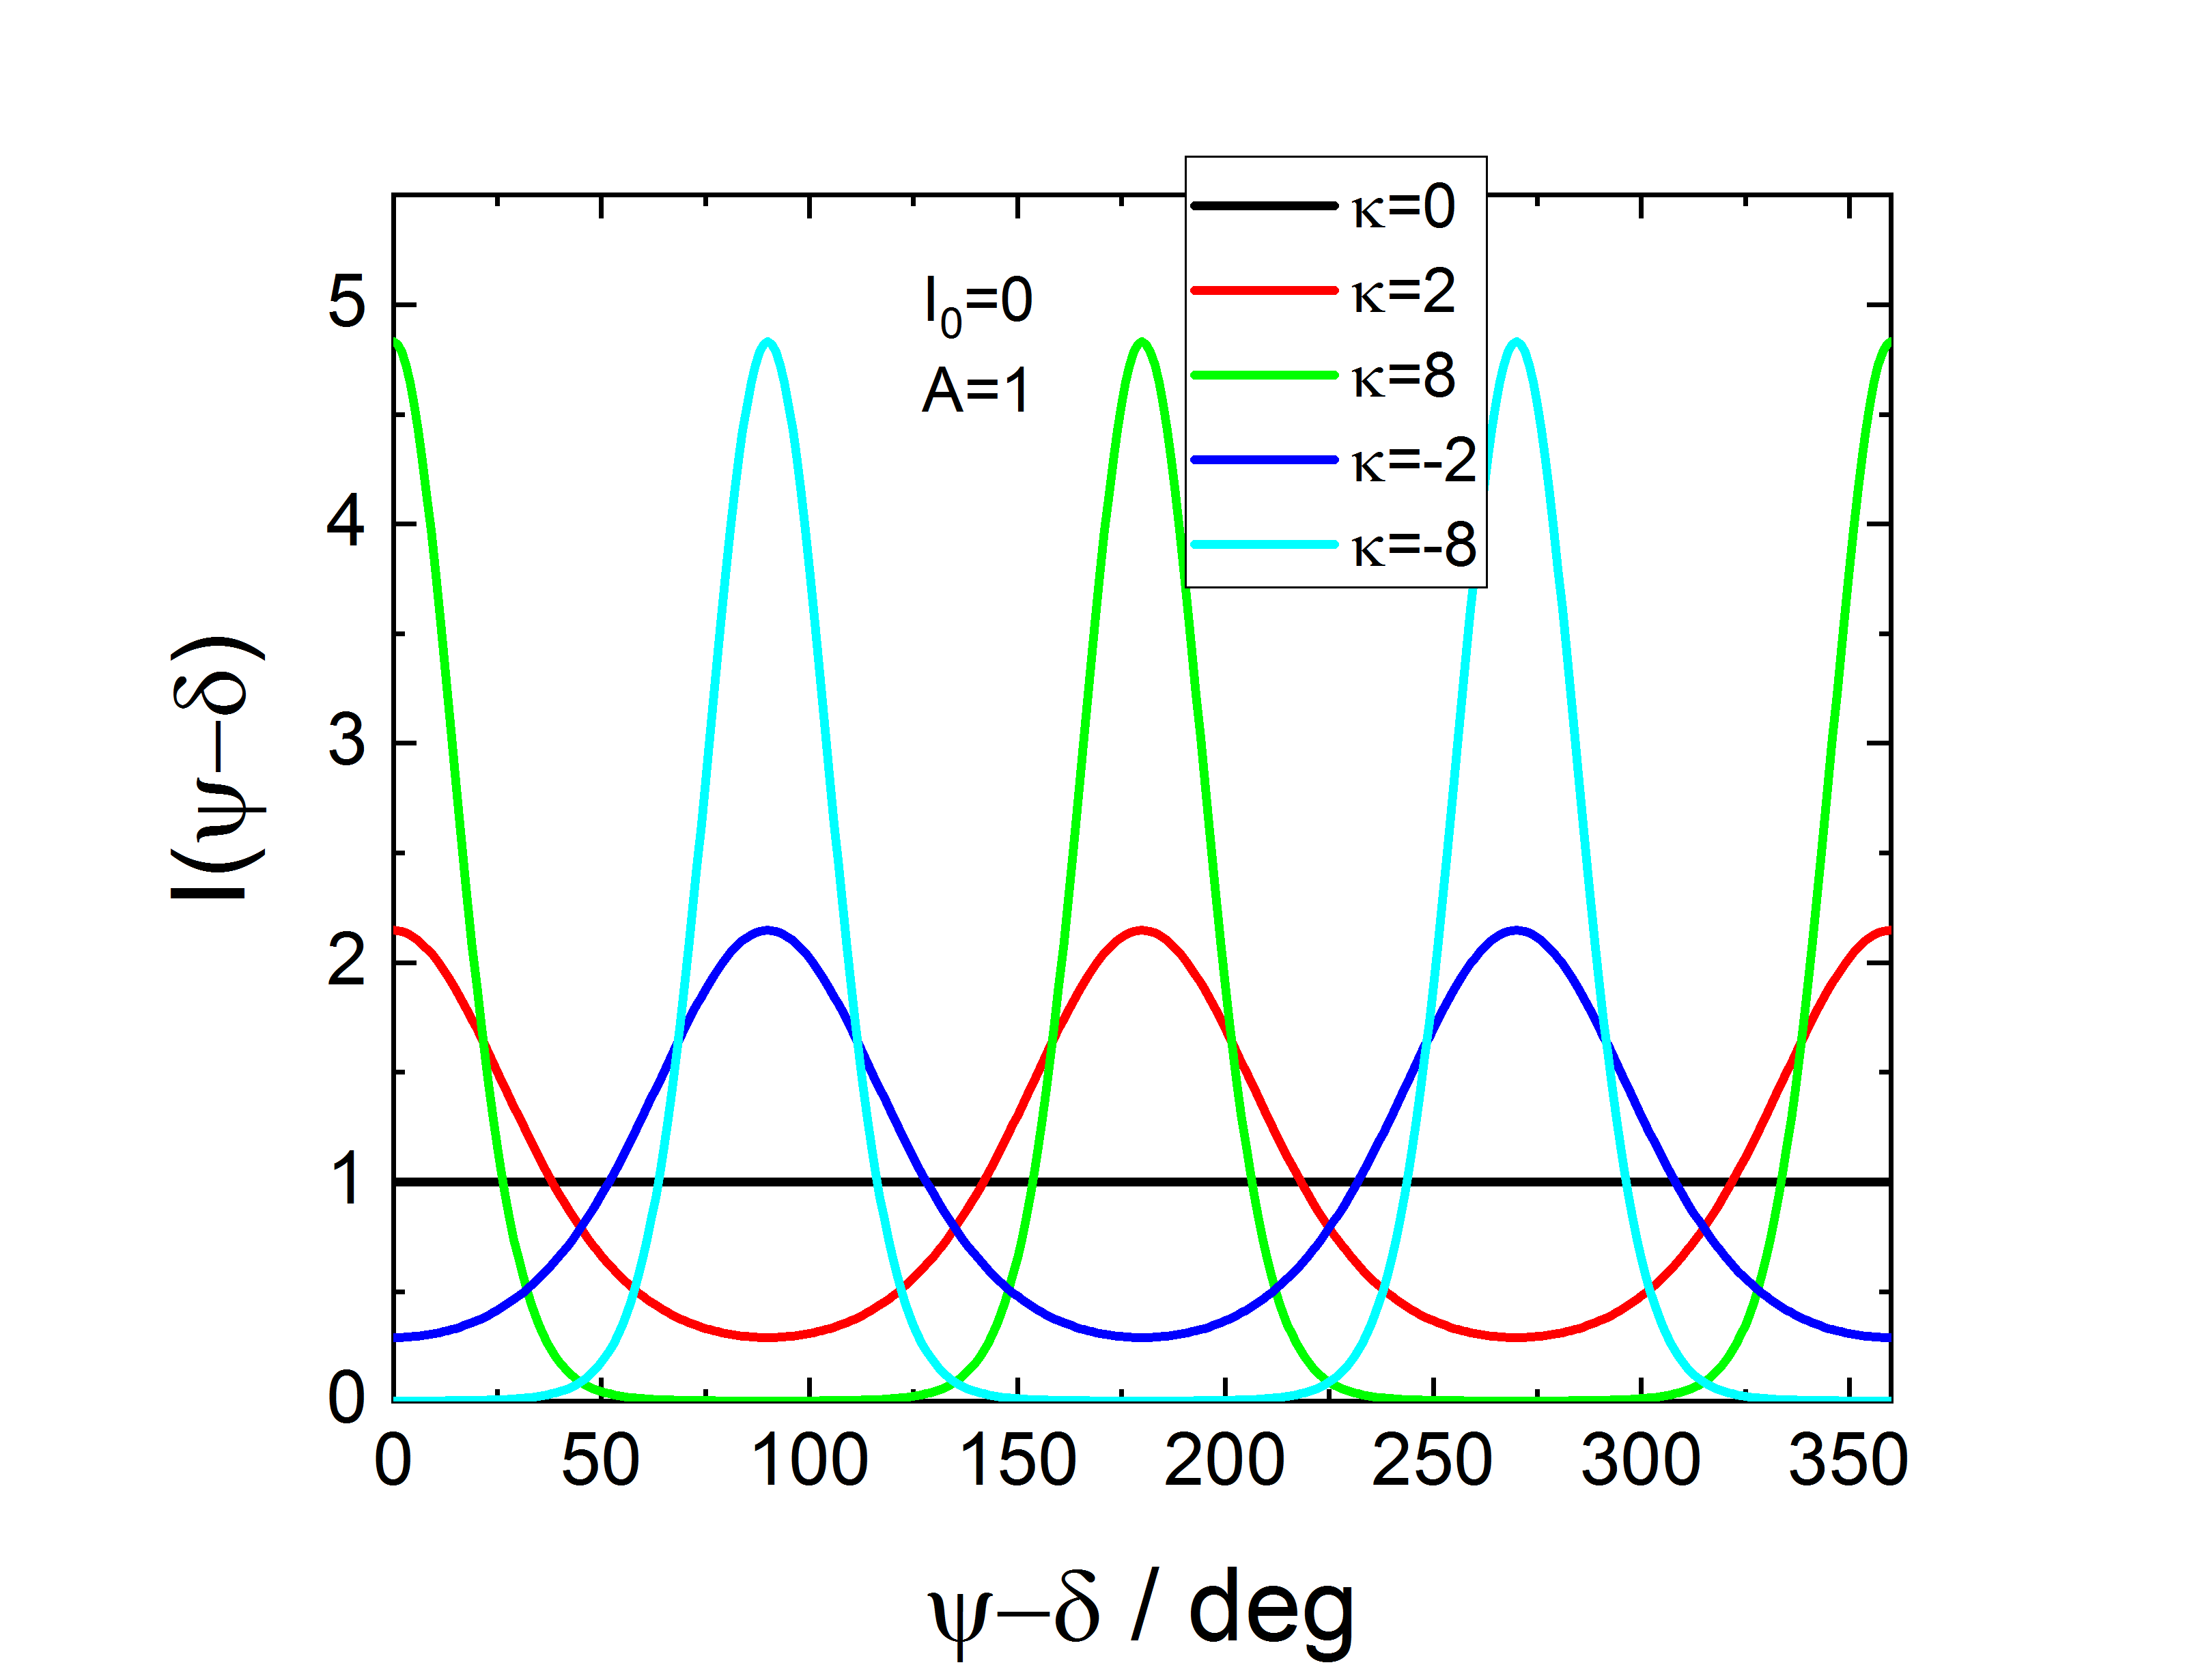
\includegraphics[width=0.7\textwidth]{../images/form_factor/azimuthal/maiersaupe.png}
\end{center}
\caption{Azimuthal intensity distribution of the Maiser-Saupe model from Picken \cite{Picken1990}}
\label{fig:maiersaupe}
\end{figure}

\subsection{affine shrinkage} ~\\
An affine deformation  profile has been given by \cite{Vilcinskas2015,Zlopasa2015} and reads as
\begin{align}
\mathcal{I}_\mathrm{as}(\psi) &= \lambda^2\frac{\cos^2\left[\arctan\left(\lambda \tan \chi\right)\right]}{\cos^3(\chi)} \\
\chi &= \psi-\delta
\end{align}
where $\lambda$ is the degree of compression. The final model function is than normalized on the average intensity so that the azimuthal intensity distribution is given by
\begin{align}
  I_\mathrm{as}(\chi) &= I_0 + A \frac{\pi}{2}\frac{\mathcal{I}_\mathrm{as}(\chi)}{\int_0^{\pi/2}\mathcal{I}_\mathrm{as}(\chi)\mathrm{d}\chi}
\end{align}

\hspace{1pt}\\
\underline{Input Parameters for models \texttt{affine shrinkage (deg)} and \texttt{affine shrinkage (rad)}:}\\
\begin{description}
\item[\texttt{I0}] flat background $I_0$
\item[\texttt{A}] Amplitude $A$ of the angle dependent intensity 
\item[\texttt{lambda}] shrinkage factor $\lambda$
\item[\texttt{delta}] direction of the polarisation $\delta$ in degree or radian
\end{description}

\underline{Note:}
$\lambda$ needs to be a positive nonzero number. $\lambda=1$: no shrinkage, $\lambda>1$: shrinkage, $0<\lambda<1$: swelling.


\begin{figure}[htb]
\begin{center}
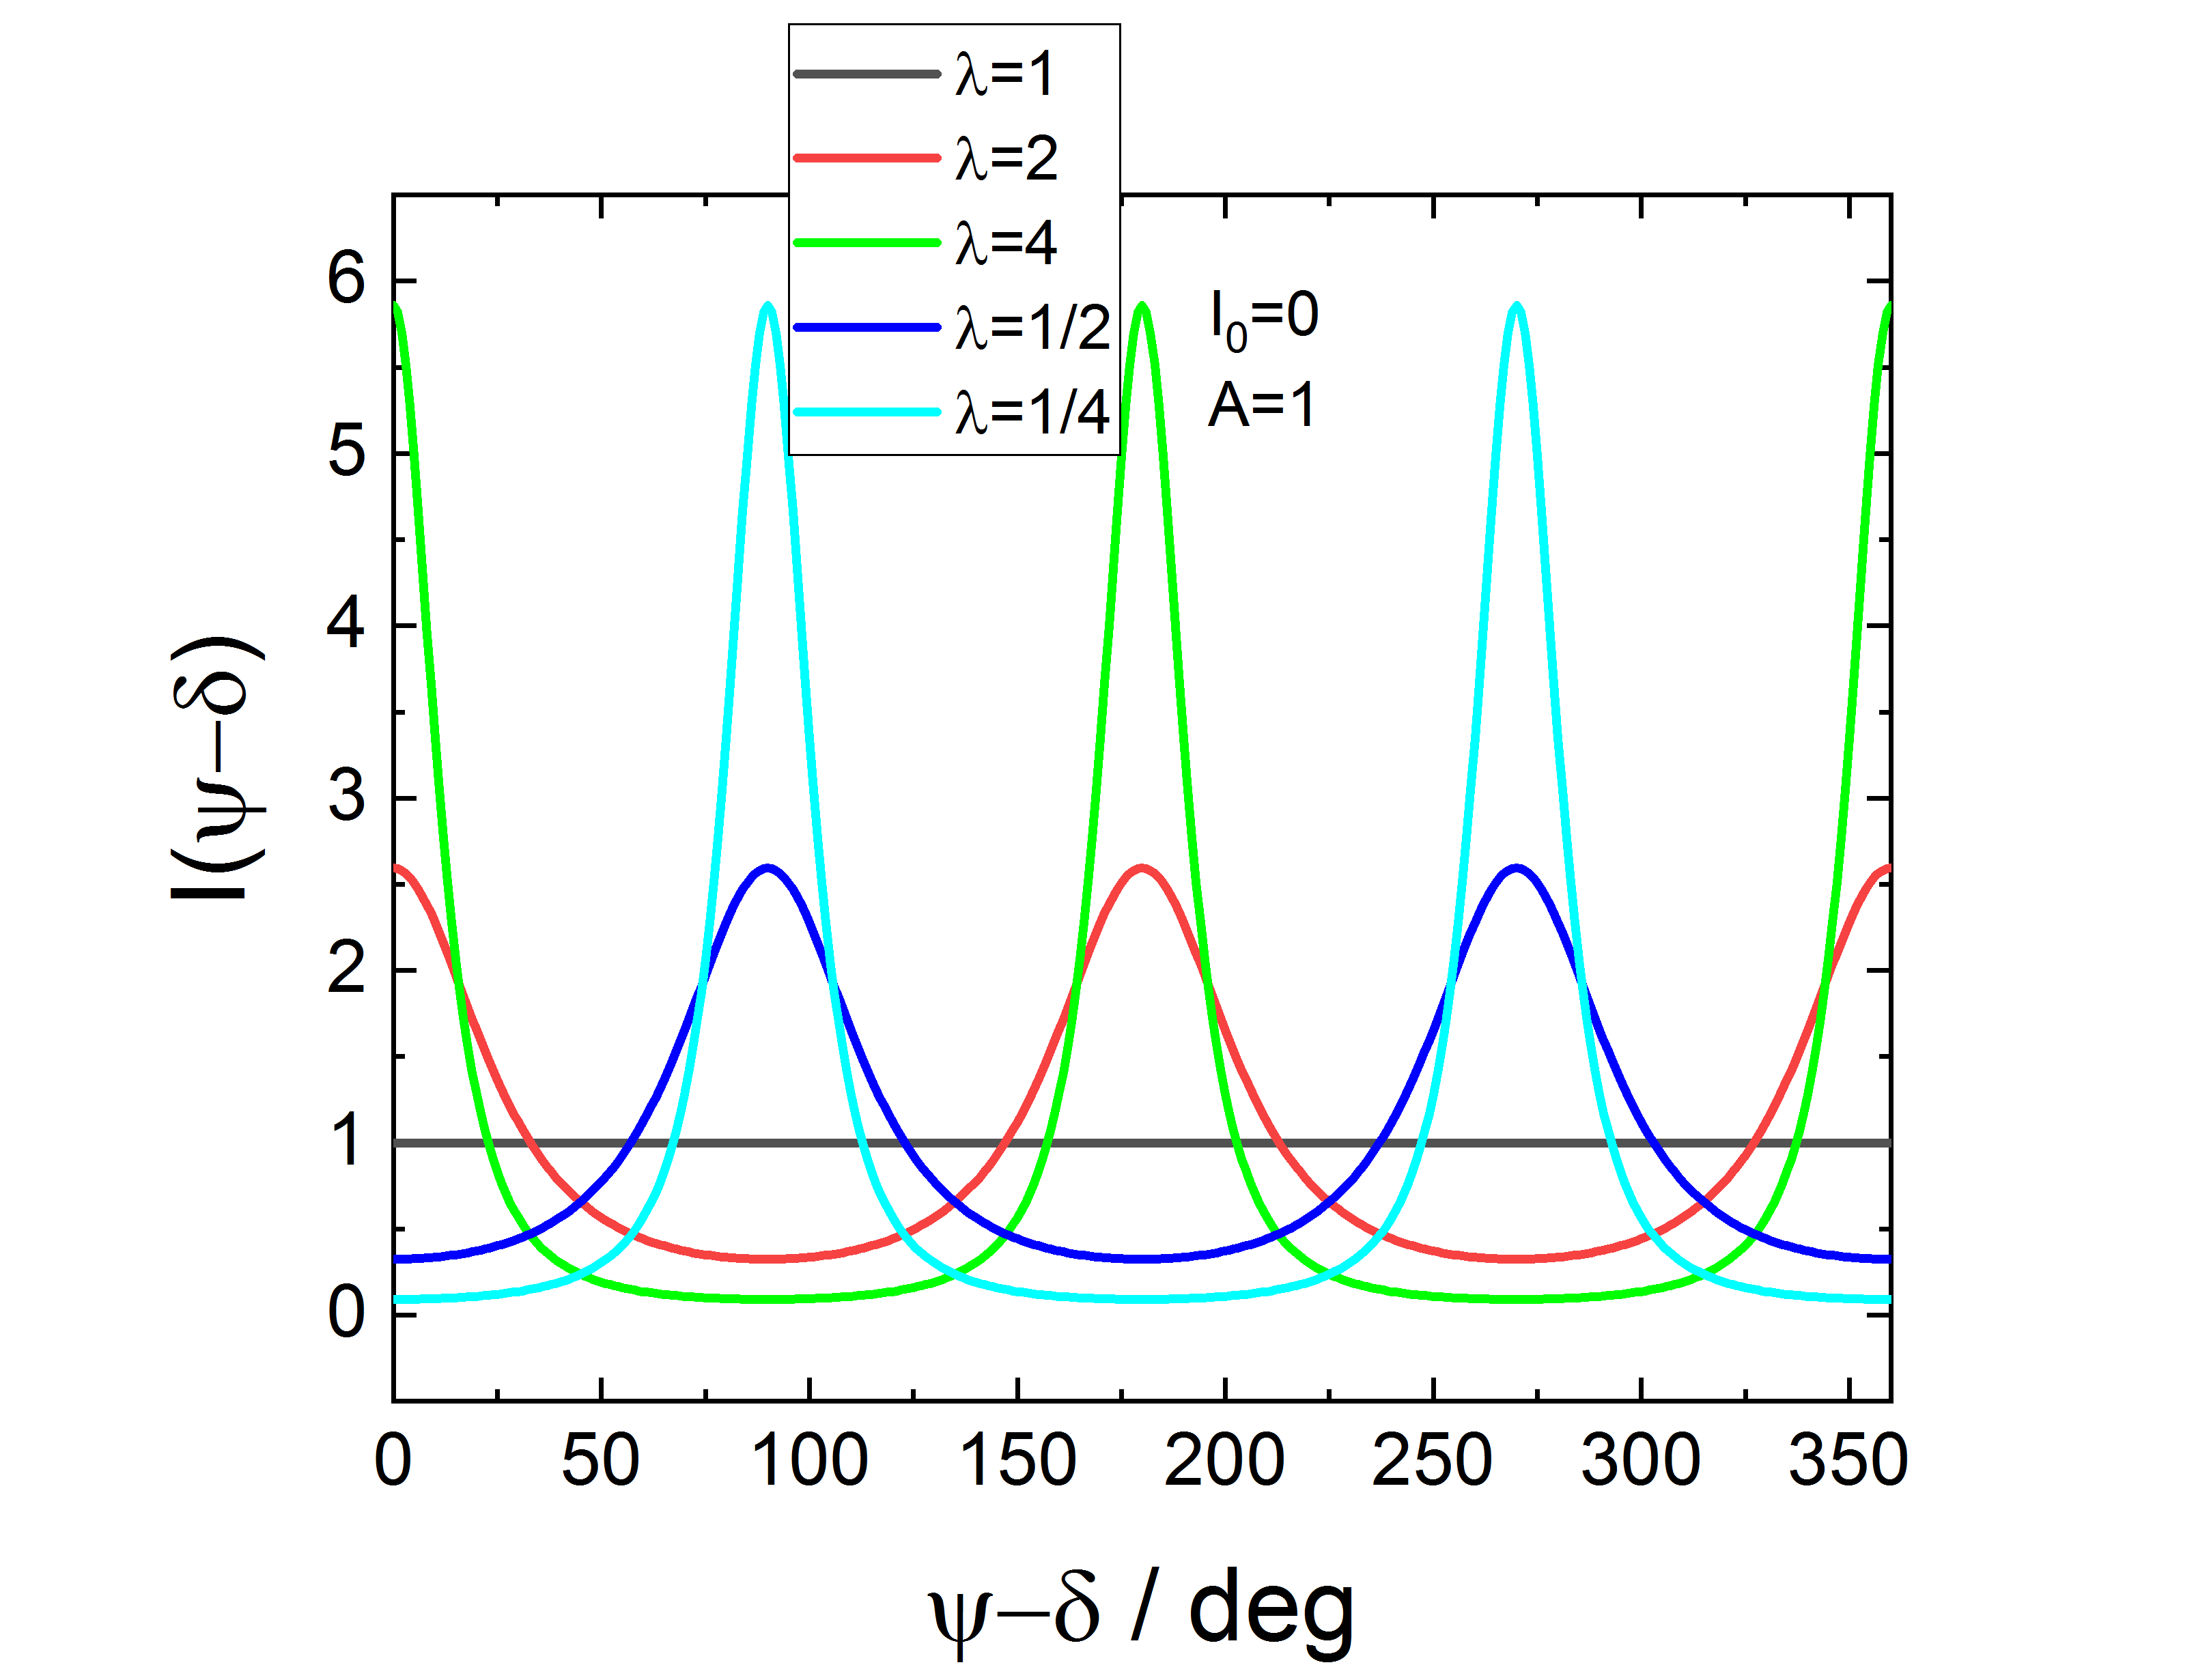
\includegraphics[width=0.7\textwidth]{../images/form_factor/azimuthal/affine_shrinkage.png}
\end{center}
\caption{Azimuthal intensity distribution of the affine shrinkage model}
\label{fig:affineshrinkage}
\end{figure}

\subsection{azimuthal analysis of very long oriented structures with Maier-Saupe or Onsager orientation distribution} ~\\
X-ray scattering has been used to obtain order parameters of liquid crystals. A work of Leadbetter and Norris \cite{Leadbetter1979} describe the underlying assumptions and derived the equation
\begin{align}
\mathcal{I}_\mathrm{LN}(\chi) &= \int_{\theta=\chi}^{\pi/2} \frac{p(\theta) \sin\theta}{\cos^2\chi \sqrt{\tan^2\theta-\tan^2\chi}} \mathrm{d}\theta
\end{align}
where $p(\theta) \sin\theta$ describe the orientation distribution of the molecular axis towards the preferred direction $\theta$. Later on it was recognized by Burger and Ruland \cite{Burger2006} that the formula contains an error and has to be corrected according to an equation derived earlier by Kratky \cite{Kratky1933}. The correct equation  which was also re-derived by Mills \cite{Mills2008} reads as \cite{Sims2018,Agra-Kooijman2017}
\begin{align}
\mathcal{I}_\mathrm{K}(\chi) &= \int_{\theta=\chi}^{\pi/2} \frac{p(\theta) \sin\theta}{\sqrt{\cos^2\chi-\cos^2\theta}} \mathrm{d}\theta = \int_{\theta=\chi}^{\pi/2} \frac{p(\theta) \sin\theta}{\sqrt{\sin^2\theta-\sin^2\chi}} \mathrm{d}\theta\\
&= \int_{\theta=\chi}^{\pi/2} \frac{p(\theta) \tan\theta}{\cos\chi \sqrt{\tan^2\theta-\tan^2\chi}} \mathrm{d}\theta
\end{align}
with $\chi = \psi-\delta$.  The final model function is than normalized on the average intensity so that the azimuthal intensity distribution is given by
\begin{align}
  I_\mathrm{LN}(\chi) &= I_0 + A \frac{\pi}{2}\frac{\mathcal{I}_\mathrm{LN}(\chi)}{\int_0^{\pi/2}\mathcal{I}_\mathrm{LN}(\chi)\mathrm{d}\chi} \\
  I_\mathrm{K}(\chi) &= I_0 + A \frac{\pi}{2}\frac{\mathcal{I}_\mathrm{K}(\chi)}{\int_0^{\pi/2}\mathcal{I}_\mathrm{K}(\chi)\mathrm{d}\chi}
\end{align}

\subsection{Ellipsoidal azimuthal analysis} ~\\
Instead of radial or sector averaged data this function describes azimuthal averaged data of deformed or textured samples with an anisotropic scattering pattern as described in
\cite{Summerfield1983,Mildner1983,Reynolds1984,Hammouda1986,Hammouda1986a,Saraf1989,Svetogorsky1990,Gu2016,Gu2018}
\begin{align}
I_\mathrm{rad}(\psi) &= \left(\left(\frac{\cos(\psi-\delta)}{A}\right)^2 + \left(\frac{\sin(\psi-\delta)}{B}\right)^2\right)^{-N/2} +C\\
I_\mathrm{deg}(\psi) &= \left(\left(\frac{\cos\left((\psi-\delta)\frac{\pi}{180}\right)}{A}\right)^2 + \left(\frac{\sin\left((\psi-\delta)\frac{\pi}{180}\right)}{B}\right)^2\right)^{-N/2}+C
\end{align}
